\documentclass[10pt]{beamer}
\usetheme[
%%% option passed to the outer theme
%    progressstyle=fixedCircCnt,   % fixedCircCnt, movingCircCnt (moving is deault)
  ]{Feather}
  
\usetikzlibrary{shapes,arrows}
\setbeamerfont{author}{size=\normalsize}
\setbeamerfont{institute}{size=\normalsize}
\setbeamerfont{title}{size=\fontsize{30}{36}\bfseries}
\setbeamerfont{subtitle}{size=\Large\normalfont\slshape}

%customized template for RTG title page
\setbeamertemplate{title page}{%
\begin{tikzpicture}[remember picture,overlay]
%color theme 
\fill[RTGblue]
  ([yshift=35pt]current page.south west) rectangle (current page.south east);
\fill[RTGred]
  ([yshift=32pt]current page.south west) rectangle ([yshift=35pt]current page.south east);  
\fill[RTGblue]
  ([yshift=-70pt]current page.north west) rectangle ([yshift=-35pt]current page.north east);
\fill[RTGred]
  ([yshift=-70pt]current page.north west) rectangle ([yshift=-72.5pt]current page.north east);
%Header: University of Mannheim/Heidelberg logo 
\node[anchor=north west] 
  at ([yshift=-6pt]current page.north west) (logo)
  {\parbox[t]{2.5cm}{\raggedleft%
    \usebeamercolor[fg]{titlegraphic}
\includegraphics[width=2cm]{uni-ma}}};
    
\node[anchor=north east] 
  at ([yshift=1pt]current page.north east) (logo)
  {\parbox[t]{2.5cm}{\raggedright%
    \usebeamercolor[fg]{titlegraphic}
\includegraphics[width=2cm]{uni-hd}}};
    
\node[anchor=north]
 at([yshift=-5pt]current page.north) (header)
 {\parbox[c]{0.5\paperwidth}{\centering \fontsize{10pt}{2pt}\selectfont Probability \& Statistics Group Heidelberg-Mannheim}};
 
 %footer   
\node[anchor=south east] 
  at ([yshift=10pt]current page.south east) (rtg)
  {\parbox[c]{2cm}{\raggedright%
   \fontsize{12pt}{2pt}\selectfont \textcolor{white} {RTG 1953}}};

%\node[anchor=south west] 
%  at ([yshift=11pt]current page.south west) (dfg)
%  {\parbox[c]{2.75cm}{\raggedleft%
%   \fontsize{0pt}{2pt}\selectfont \textcolor{white} { }}};
%   
\node[anchor=south west] 
  at ([yshift = 7pt,xshift=0.28cm]current page.south west) (logo)
  {\parbox[c]{1.2cm}{\raggedleft%
   \usebeamercolor[fg]{titlegraphic}
\includegraphics[width=1.2cm]{dfg}}};
    

%% title + author, adjust yshift value if necessary (controls vertical position)
\node[anchor=center]
  at ([yshift=10pt]current page.center) (title)
  {\parbox[t]{\textwidth}{\linespread{6} \selectfont \centering%
\fontsize{14pt}{3pt}\selectfont \textcolor{black}{\inserttitle}}};
 
\node[anchor=center]
  at ([yshift=-45pt]current page.center) (author)
  {\parbox[c]{\textwidth}{\centering\usebeamerfont{author}\textcolor{black}{\insertauthor}}};
\end{tikzpicture}
}


% If you want to change the colors of the various elements in the theme, edit and uncomment the following lines
\definecolor{RTGblue}{HTML}{2E2E2E}
\definecolor{RTGred}{HTML}{C80B33}
\definecolor{black}{rgb}{0.0, 0.0, 0.0}

% Change the bar colors:
\setbeamercolor{Feather}{fg=red!80!black, bg=RTGblue}
\setbeamercolor{block title}{bg=RTGblue, fg=white}
\setbeamercolor{block body}{bg=white, fg=black}

% Change the color of the structural elements:
\setbeamercolor{structure}{fg=black}

% Change the frame title text color:
\setbeamercolor{frametitle}{fg=white}

% Change the normal text color background:
%\setbeamercolor{normal text}{fg=black,bg=gray!10}

%-------------------------------------------------------
% INCLUDE PACKAGES
%-------------------------------------------------------
\usepackage{ifpdf}
\usepackage{xcolor}
\usepackage{graphicx} 
\usepackage{multicol}
\usepackage{libertineotf}
\usepackage{tikz}
\usepackage{animate}
\usepackage{pdfrender}
\usepackage{amsmath}

\ifpdf
\DeclareGraphicsRule{*}{mps}{*}{}
\else
% Recent LaTeX versions donât require the next line
% \DeclareGraphicsRule{*}{eps}{*}{}
\fi


\usepackage[sfdefault]{AlegreyaSans} %% Option 'black' gives heavier bold face
%% The 'sfdefault' option to make the base font sans serif
\renewcommand*\oldstylenums[1]{{\AlegreyaSansOsF #1}}
    
\usepackage{natbib}
\usepackage[english]{babel}
\usepackage{caption}
\usepackage{subcaption}
\usepackage[utf8]{inputenc}
%\usepackage[TS1,T1]{fontenc}
%\usepackage{helvet}
\usepackage{fourier}
\usepackage{hyperref}
%\usepackage{lmodern}
%\usepackage{mathrsfs}
\usepackage{amsmath,amssymb,amsfonts,graphicx,shorttoc,textpos,caption,here, yfonts}
\usepackage{verbatim,enumerate,dsfont,fancyhdr,setspace,array}
\usepackage[cal=boondox]{mathalfa}

%\usepackage[style=authoryear]{biblatex}
%\renewcommand*{\nameyeardelim}{\addcomma\addspace}


\graphicspath{{Feathergraphics/}}
%\bibliography{biblio1}
%\DeclareCiteCommand{\cite}
%{\usebibmacro{prenote}}
%{\usebibmacro{citeindex}%
%\usebibmacro{cite}}
%{\multicitedelim}
%{\usebibmacro{cite:postnote}}
%\usefonttheme[onlymath]{serif}
%\newbibmacro*{cite}{%
%\usebibmacro{cite:citepages}%
%\ifciteseen
%	{\iffieldundef{shorthand}
%		{\usebibmacro{cite:short}}
%		{\usebibmacro{cite:shorthand}}}
%	{\usebibmacro{cite:full}}}
%
%\renewbibmacro*{cite}{%
%\usebibmacro{cite:citepages}%
%{\usebibmacro{cite:full}}}
%-------------------------------------------------------
% DEFFINING AND REDEFINING COMMANDS
%-------------------------------------------------------

% colored hyperlinks
\newcommand{\chref}[2]{
  \href{#1}{{\usebeamercolor[bg]{Feather}#2}}
}
\DeclareMathOperator*{\argmin}{arg\,min}
%\bibliographystyle{apalike}
%\renewcommand\bibfont{\scriptsize}
\DeclareMathOperator*{\Argmin}{Arg\,min}
\setbeamertemplate{frametitle continuation}[from second]

%-------------------------------------------------------
% INFORMATION IN THE TITLE PAGE
%-------------------------------------------------------

\title[Frequentist and Bayesian methods for ill-posed inverse problems] % [] is optional - is placed on the bottom of the sidebar on every slide
{ % is placed on the title page
     \textbf{Frequentist and Bayesian methods for ill-posed inverse problems}
}


\subtitle[loizeau@math.uni-heidelberg.de] % [] is optional - is placed on the bottom of the sidebar on every slide
{}


\institute[Ruprecht-Karls-Universität Heidelberg]
{

  \begin{flushright}Ruprecht-Karls-Universität Heidelberg\end{flushright}
  %there must be an empty line above this line - otherwise some unwanted space is added between the university and the country (I do not know why;( )
}

\date{}

\author[Xavier Loizeau] % [] is optional - is placed on the bottom of the sidebar on every slide
{Oracle and minimax optimality
}
%-------------------------------------------------------
% THE BODY OF THE PRESENTATION
%-------------------------------------------------------

\begin{document}
%-------------------------------------------------------
% THE TITLEPAGE
%-------------------------------------------------------

% % this is the name of the PDF file for the background
\begin{frame}[plain,noframenumbering] % the plain option removes the header from the title page, noframenumbering removes the numbering of this frame only
  \titlepage % call the title page information from above
\end{frame}

\AtBeginSection[]{
\begin{frame}[noframenumbering]{Contents}
\setcounter{tocdepth}{1}
%\begin{multicols}{2}
\tableofcontents[sectionstyle=show/shaded, subsectionstyle=show/show/hide]
%\end{multicols}
\end{frame}
}

\begin{frame}{Contents}
\setcounter{tocdepth}{1}
\tableofcontents
\end{frame}

\section{Statistical estimation, frequentist versus Bayesian approach}

\begin{frame}{Frequentist estimation, mainstay}
\includegraphics<1>[scale=.8]{est-freq/freq-est.1}
\includegraphics<2>[scale=.8]{est-freq/freq-est.2}
\includegraphics<3>[scale=.8]{est-freq/freq-est.3}
\includegraphics<4>[scale=.8]{est-freq/freq-est.4}
\end{frame}

\begin{frame}{Frequentist estimation, data example}
\begin{figure}
\centering
 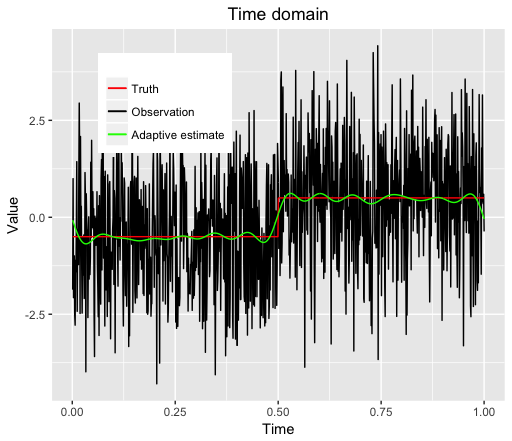
\includegraphics[width=.75\linewidth]{freq_est.png}
\caption{Estimating the drift in a Gaussian precess by aggregation of projection estimators}\label{freq_est}
\end{figure}
\end{frame}

\begin{frame}{Frequentist estimation, mathematical formulation}
\begin{alignat*}{3}
& dY_{x} &&=&& \theta^{\circ}_{x} dx + \frac{1}{\sqrt{n}} dW(x);\\
& Y_{j} &&=&& \mathcal{F}(Y)(j) = \mathcal{F}(\theta^{\circ})(j) + \frac{1}{\sqrt{n}} \xi_{j};\\
& \xi_{j} && \sim_{iid} && \mathcal{N}(0,1);\\
& \widehat{\theta}_{j} &&=&& \mathds{1}_{j \leq m} Y_{j};\\
& \widetilde{\theta}_{x} &&=&& \mathcal{F}^{-1}(\widehat{\theta})(x).
\end{alignat*}
\end{frame}

\begin{frame}{Bayesian estimation, mainstay}
\includegraphics<1>[scale=.8]{est-bayes/bayes-est.1}
\includegraphics<2>[scale=.8]{est-bayes/bayes-est.2}
\end{frame}

\begin{frame}{Bayesian estimation, data example}
\begin{figure}
\centering
 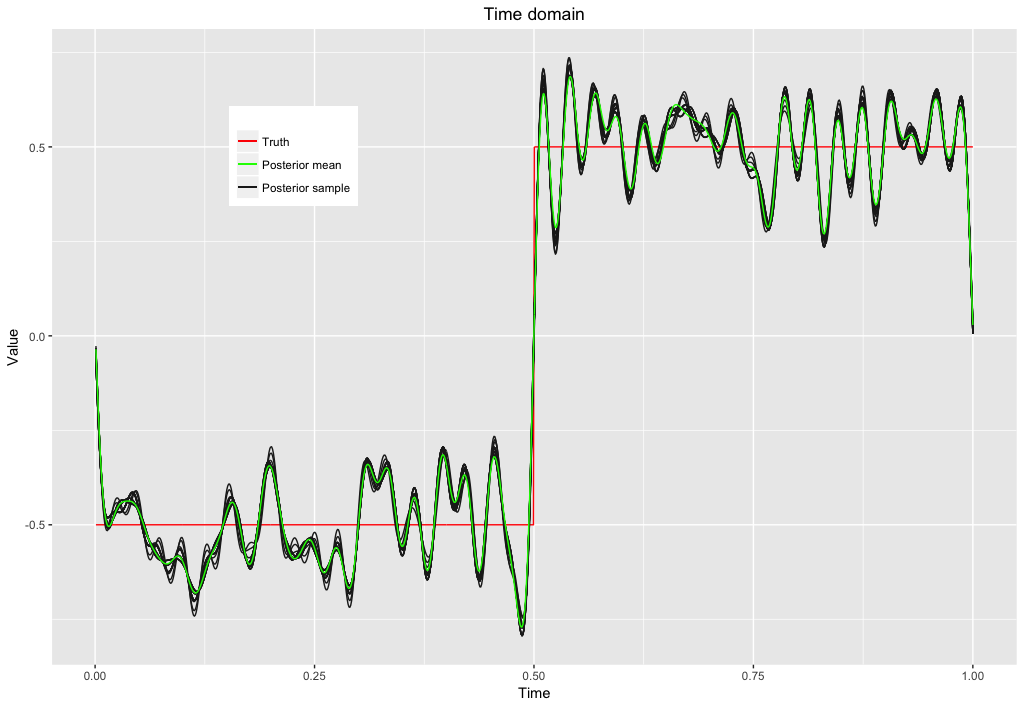
\includegraphics[width=.75\linewidth]{sample_bayes.png}
\caption{Sample from the posterior distribution of a hierarchical sieve prior}\label{sample_bayes}
\end{figure}
\end{frame}

\begin{frame}{Bayesian estimation, mathematical formulation}
\begin{alignat*}{3}
& \boldsymbol{\theta}_{j} &&\sim&& \mathcal{N}(0, 1) \mathds{1}_{j \leq m} + \delta_{0}\mathds{1}_{j > m};\\
& Y_{j}\vert \boldsymbol{\theta}_{j} &&\sim&& \mathcal{N}(\boldsymbol{\theta}, \frac{1}{n});\\
& \boldsymbol{\theta}_{j} \vert Y_{j} &&\sim&& \mathcal{N}(\widehat{\theta}_{j}, \sigma_{j}) \mathds{1}_{j \leq m} + \delta_{0}\mathds{1}_{j > m};\\
& \widehat{\theta}_{j} &&=&& \frac{n \cdot Y_{j}}{1 + n};\\
& \sigma_{j} &&=&& \frac{1}{1 + n}.
\end{alignat*}
\end{frame}

\section{Ill-posed inverse problems}

\begin{frame}{Ill posed-inverse problems, mainstay}
\includegraphics<1>[scale=.8]{inv-prob/inv-prob.1}
\includegraphics<2>[scale=.8]{inv-prob/inv-prob.2}
\includegraphics<3>[scale=.8]{inv-prob/inv-prob.3}
\includegraphics<4>[scale=.8]{inv-prob/inv-prob.4}
\includegraphics<5>[scale=.8]{inv-prob/inv-prob.5}
\includegraphics<6>[scale=.8]{inv-prob/inv-prob.6}
\includegraphics<7>[scale=.8]{inv-prob/inv-prob.7}
\includegraphics<8>[scale=.8]{inv-prob/inv-prob.8}
\includegraphics<9>[scale=.8]{inv-prob/inv-prob.9}
\includegraphics<10>[scale=.8]{inv-prob/inv-prob.10}
\includegraphics<11>[scale=.8]{inv-prob/inv-prob.11}
\includegraphics<12>[scale=.8]{inv-prob/inv-prob.12}
\includegraphics<13>[scale=.8]{inv-prob/inv-prob.13}
\end{frame}

\begin{frame}{Ill posed-inverse problems, data example}
	\begin{center}
		\animategraphics[loop,controls,width=40ex]{10}{animation/test-}{0}{147}
	\end{center}
\end{frame}

\begin{frame}{Ill posed-inverse problems, mathematical formulation}
	\begin{alignat*}{4}
		& \text{Process: }&&\frac{\partial Y_{x, t}}{\partial t} &&=&& \frac{\partial^{2} Y_{x, t}}{\partial x^{2}} + \frac{1}{n} \frac{dW (x, t)}{dt};\\
		& \text{Solution: }&& Y_{j}(t) &&=&& \theta^{\circ}_{j}(t) + \frac{1}{n} \xi_{j}(t)\\
		& && \theta^{\circ}_{j}(t) &&=&& \mathcal{F}(\theta^{\circ}(\cdot, 0))(j) \cdot \exp[-j^{2} t]\\
		& \text{Observation: }&&Y_{j} &&=&& \theta^{\circ}_{j}(T) + \frac{1}{n} \xi_{j};\\
		& \text{Interest: }&&\theta^{\circ}_{j}(0) && = && \theta^{\circ}_{j}(T)\exp[j^{2} T].
\end{alignat*}
\end{frame}

\section{Quantification of the quality of a statistical method}
\begin{frame}{Frequentist convergence rate, mainstay}
\begin{columns}[c]
	\begin{column}{3cm}
		\includegraphics<1>[scale=.8]{convergence-rate/convergence-rate.1}
		\includegraphics<2>[scale=.8]{convergence-rate/convergence-rate.2}
		\includegraphics<3>[scale=.8]{convergence-rate/convergence-rate.3}
		\includegraphics<4>[scale=.8]{convergence-rate/convergence-rate.4}
		\includegraphics<5>[scale=.8]{convergence-rate/convergence-rate.5}
	\end{column}
	\begin{column}{8cm}
		\begin{itemize}
			\item<1-> Distance to the truth:
			\[l(\widehat{\theta}, \theta^{\circ})\]
			\item<2-> Average distance to the truth:
			\[\mathds{E}_{\theta^{\circ}}\left[l(\widehat{\theta}, \theta^{\circ})\right]\]
			\item<3-> Lower bound: $\Phi_{n}(\theta^{\circ}) \rightarrow 0$, $K > 1$
			\[ \inf\limits_{\widetilde{\theta} \in \mathcal{E}}\mathds{E}_{\theta^{\circ}}\left[l(\widetilde{\theta}, \theta^{\circ})\right] \geq K^{-1} \Phi_{n}(\theta^{\circ}).\]
			Upper bound:
			\[\mathds{E}_{\theta^{\circ}}\left[l(\widehat{\theta}, \theta^{\circ})\right] \leq K \Phi_{n}(\theta^{\circ}).\]
		\end{itemize}
	\end{column}
\end{columns}
\end{frame}

\begin{frame}{Frequentist convergence rate, example}
\begin{itemize}\centering
\item<1|only@1> $\Vert \widehat{\theta} - \theta^{\circ} \Vert^{2} = \int\limits_{[0,1]} (\widehat{\theta}(x) - \theta^{\circ}(x))^{2} dx;$
\item<2|only@2> $\mathds{E}_{\theta^{\circ}}[\Vert \widehat{\theta} - \theta^{\circ} \Vert^{2}] = \int\limits_{X} \Vert \widehat{\theta}(Y^{n}) - \theta^{\circ} \Vert d\mathds{P}_{Y^{n}};$
\item<3|only@3> $\mathds{E}_{\theta^{\circ}}[\Vert \widehat{\theta} - \theta^{\circ} \Vert^{2}] = \mathcal{O}_{n}(\Phi^{\circ}_{n})$
\end{itemize}
\vfill
\begin{figure}
 \includegraphics<1>[width=.75\linewidth]{error.pdf}
 \includegraphics<2>[width=.75\linewidth]{error_density.pdf}
 \includegraphics<3>[width=.75\linewidth]{error_evol.pdf}
\end{figure}
\end{frame}

\begin{frame}{Bayesian contraction rate, principle}
\begin{columns}[c]
	\begin{column}{3cm}
\includegraphics<1>[scale=.8]{contraction-rate/contraction-rate.1}
\includegraphics<2>[scale=.8]{contraction-rate/contraction-rate.1}
\includegraphics<3>[scale=.8]{contraction-rate/contraction-rate.2}
\includegraphics<4>[scale=.8]{contraction-rate/contraction-rate.3}
\includegraphics<5>[scale=.8]{contraction-rate/contraction-rate.4}
\includegraphics<6>[scale=.8]{contraction-rate/contraction-rate.5}
	\end{column}
	\begin{column}{8cm}
		\begin{itemize}
			\item<1-> Probability to give a guess within a distance of the truth:
			\[\mathds{P}_{\boldsymbol{\theta} \vert Y^{n}}\left(\boldsymbol{\theta} : l(\boldsymbol{\theta}, \theta^{\circ}) \leq \Phi_{n}\right);\]
			\item<2->  Average probability to give a guess within a distance of the truth:
			\[\mathds{E}_{\theta^{\circ}}[\mathds{P}_{\boldsymbol{\theta} \vert Y^{n}}\left(\boldsymbol{\theta} : l(\boldsymbol{\theta}, \theta^{\circ}) \leq \Phi_{n}\right)];\]
			\item<3-> Lower bound:
			\[\lim\limits_{n \rightarrow \infty} \sup\limits_{\mathds{Q}_{\boldsymbol{\theta}} \in \mathcal{G}} \mathds{E}_{\theta^{\circ}}[\mathds{P}_{\boldsymbol{\theta} \vert Y^{n}}\left(\boldsymbol{\theta} : l(\boldsymbol{\theta}, \theta^{\circ}) \leq K^{-1} \Phi_{n}\right)] < 1;\]
			upper bound:
			\[\lim\limits_{n \rightarrow \infty}\mathds{E}_{\theta^{\circ}}[\mathds{P}_{\boldsymbol{\theta} \vert Y^{n}}\left(\boldsymbol{\theta} : l(\boldsymbol{\theta}, \theta^{\circ}) \leq K \Phi_{n}\right)] = 1.\]
		\end{itemize}
	\end{column}
\end{columns}
\end{frame}

\begin{frame}{Bibliography}
\bibliography{iGSSM.bib}{}
\end{frame}
\nocite{*}
\bibliographystyle{apalike}

\end{document}